\label{s:filtering_monogenic}
%
\comment{If we need the space, I'd consider reducing this to a paragraph that states that the monogenic signal suffers the same problems as first derivatives, despite its use of phase.}
%
\begin{figure}[t]
\centering
\begin{tabular}{@{}c c c@{}} % @{} removes padding around the edge of the table
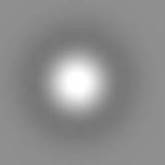
\includegraphics[width=0.2\columnwidth]{\figpath/filtering/mono_b} &
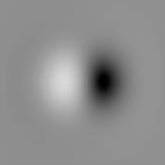
\includegraphics[width=0.2\columnwidth]{\figpath/filtering/mono_hx} &
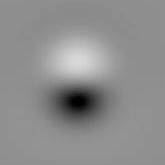
\includegraphics[width=0.2\columnwidth]{\figpath/filtering/mono_hy} \\
(a) & (b) & (c)
\end{tabular}
%
\caption{Monogenic signal filters (a) $B$, (b) $h_x$, and (c) $h_y = h_x^T$.}
\label{f:filters_monogenic}
\end{figure}
%
The monogenic signal~\cite{Felsberg_Sommer_TSP01} computes phase and orientation at a given image location using three filters: one even band-pass filter $B$, and an odd quadrature pair of filters $h_x(x,y) = x/f(x,y)$ and $h_y(x,y) = y/f(x,y)$ where $f(x,y) = 2\pi(x^2 + y^2)^{\frac{3}{2}}$ (\fref{f:filters_monogenic}). These filters are combined to compute local amplitude~($A$), phase~($\psi$) and orientation~($\theta$) at every location in the image:

\begin{align}
A       &= \sqrt{{I_B}^2 + {I_{hx}}^2 + {I_{hy}}^2} 
\label{e:monogenic_amplitude} \\
%
\psi	  &= \tan^{-1}\left[ \frac{I_B}{\sqrt{{I_{hx}}^2 + {I_{hy}}^2}} \right]
\label{e:monogenic_phase} \\
%
\theta  &= \tan^{-1}\left[ \frac{I_{hy}}{I_{hx}} \right] 
\label{e:monogenic_orientation}
\end{align}

\noindent where $I_B = I \ast B$, $I_{hx} = h_x \ast I_B$ and $I_{hy} = h_y \ast I_B$.

The local amplitude provides a magnitude of response that is consistent for all structures and orientations while the local phase provides a measure of symmetry (in a profile of the structure perpendicular to its orientation), varying from $-\pi/2$ for a negative line (\ie~a dark line on a light background), through $0$ for an edge, to $\pi/2$ for a positive line.

Though the monogenic signal combines both odd and even filters, the even filter $B$ is isotropic and therefore has no directional sensitivity. All orientation information therefore comes from the odd filters $h_x$ and $h_y$, such that orientation is not recovered for symmetric image features (\eg~at the centre of a bar or ridge).
